\chapter{Aplicaciones a la biología}

En este capítulo, introduciremos algunos problemas de biología computacional y de bioinformática que pueden ser resueltos mediante el uso de HMM. Empezaremos presentado algunos conceptos básicos de biología relacionados con nuestro estudio, discutiremos sobre la naturaleza y la importancia que tienen los problemas y cómo podemos adaptar el modelo y los algoritmos vistos en el capítulo anterior para resolverlos.

Para este capítulos, las fuentes principales son \cite{Durbin}, \cite{Yoon} y \cite[Capítulo 8]{Vidyasagar}.

\section{Nociones básicas de biología}
Para nuestro estudio necesitamos introducir algunas nociones básicas de biología, en concreto, presentaremos conceptos relacionados con el ADN y las proteínas. Cabe destacar que por el carácter que tiene este trabajo, no entraremos en detalle sobre estos conceptos y sólo vamos a exponer la información relevante para poder introducir los problemas. Por lo tanto, el lector puede encontrar en determinadas ocasiones, un falta de rigor en el sentido de biología. Por último, este apartado se basa esencialmente en \cite[Capítulo 8]{Vidyasagar} y \cite[Apéndice A]{Warren}.

El material genético para la mayoría de los seres vivos es el ácido desoxirribonucleico, conocido generalmente como ADN. Consiste en un polímero (conjunto) de nucleótidos, en los que cada nucleótido está compuesto por un glúcido (la desoxirribosa), un grupo fosfato y una base nitrogenada de uno de los siguientes cuatro tipos: adenina, guanina, citosina y timina. En general, se denota a cada nucleótido por la letra inicial de la base que contiene, es decir, por $A,\, G,\, C$ y $T$ respectivamente. 

Nucleótidos adyacentes en una de las cadenas del ADN se conectan mediante un vínculo químico entre el glúcido de uno y el grupo fosfato del siguiente. La estructura clásica de doble hélice del ADN se forma cuando se conectan las dos cadenas de nucleótidos mediante puentes de hidrógeno. Estas conexiones sólo se forman para pares de nucleótidos concretos (conocidos como par de bases): la adenina con la timina ($A\leftrightarrow T$) y la guanina con la citosina ($G\leftrightarrow C$). Por lo tanto, las dos cadenas de ADN son complementarias pues si una cadena contiene una $A$, entonces estará conectada con una $T$ en la cadena contraria. Análogamente, si una contiene una $C$, la otra contendrá una $G$. 

\begin{figure}[H]
    \centering
    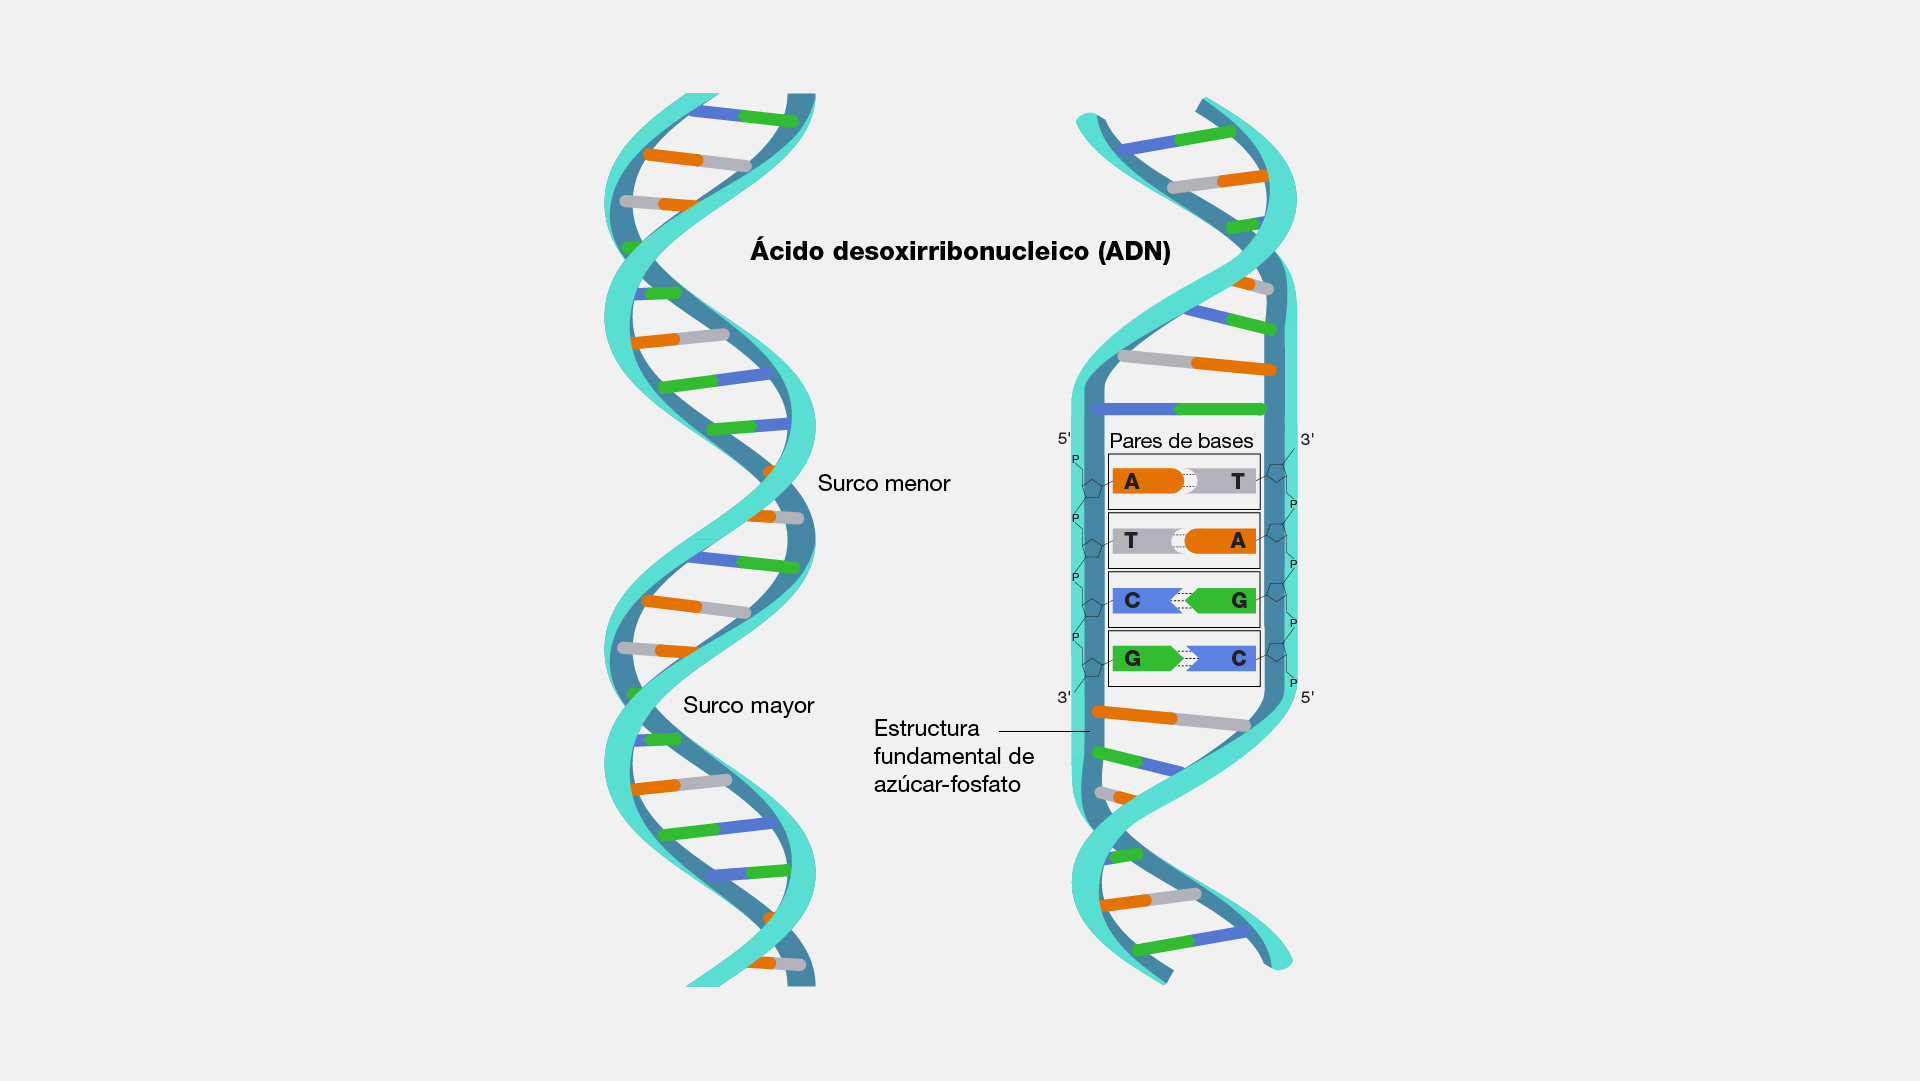
\includegraphics[width=\textwidth]{img/Estructura_del_ADN.jpg}
    \caption{Estructura del ADN \cite{genome}}
\end{figure}

La secuencia en la que constituyen las diferentes bases en una de las cadenas del ADN representa la información genética codificada en dicha cadena. Por la complementariedad de las cadenas, a partir de una de ellas se puede también determinar la información de la otra. Además, cada cadena tiene definida una dirección espacial contraria a la otra, de modo que sólo podemos interpretar una cadena en la dirección correspondiente.

A nivel celular, el ADN se organiza en cromosomas, cada uno de los cuales contiene un ADN que puede tener cientos de millones de par de bases. La mayoría de las células humanas contienen 23 pares de cromosomas, uno heredado del padre y el otro de la madre. Los dos cromosomas de un par son prácticamente idénticos, con la excepción del cromosoma sexual, para el cual existen dos tipos, X e Y. Casi todas las células del cuerpo humano contienen copias idénticas del conjunto completo de 23 pares de cromosomas. El conjunto total de ADN de un organismo se conoce como su genoma, cabe destacar que el genoma humano contiene a más de tres mil millones de pares de bases.

Un cromosoma humano está compuesto principalmente por ADN no codificante, cuya función apenas se está empezando a entender. Interpuesto en el ADN se encuentran genes que codifican proteínas. Estos genes representan aproximadamente el $2\%$ del genoma humano, sin embargo, son el foco de atención de los genetistas. Los genes a menudo están organizados en exones, que son secuencias que eventualmente serán utilizadas por la célula, alternado con intrones, que serán descartados en el proceso de codificación. La información en estos genes se codificará en ARN (ácido ribonucleico), y en muchos casos, finalmente en proteínas.

En el proceso de codificación de un gen a un ARN, se utiliza la secuencia de ADN del gen (eliminano los intrones) como plantilla. Al igual que el ADN, el ARN está también compuesto por una serie de nucleótidos, pero con ciertas diferencias: el ARN está formado en general por una única cadena y sustituye la base nitrogenada uracilo ($U$) por la timina ($T$). Un caso particular de ARN, el ARNm (ARN mensajero), será finalmente transformado en proteína.

Una proteína está compuesta por una secuencia de aminoácidos, existen una gran variedad de aminoácidos pero sólo $20$ aparecen en las proteínas. Cada uno de estos aminoácidos está representado por una o más secuencias de tres nucleótidos de ARN conocidas como codones. La combinación de cuatro posibles nucleótidos en grupos de tres resulta en $4^3=64$ codones, lo que significa que la mayoría de los aminoácidos están codificados por más de un codón. La función de una proteína depende finalmente tanto de su secuencia de aminoácidos como de la estructura tridimensional que ha adquirido de su transformación a partir de un ARNm. 

\section{Software utilizado}
Antes de presentar las aplicaciones de HMM en la biología, presentamos los recursos software que vamos a utilizar para ilustrar algunos ejemplos. Como recurso principal se va a utilizar dos librerías de Python:
\begin{itemize}
    \item \textbf{NumPy}: es una de las librerías más utilizadas de Python, proporciona la capacidad de tratar elementos matemáticos de forma sencilla y eficiente. En este caso se ha utilizado la versión más reciente hasta el momento, la 1.24.3. Se puede consultar la documentación en \cite{numpy}.
    \item \textbf{hmmlearn}: es una librería de códigos abiertos para Python que implementa modelos de Markov ocultos. Utiliza códigos escrito en C++ para los algoritmos, de forma que son más eficientes que si son implementados directamente en Python. También implementa modelos que no hemos visto en este trabajo. Se ha utilizado para este trabajo la versión 0.3.0. Se puede consultar la documentación en \cite{hmmlearn} y el código en \cite{hmmlearnGithub}
\end{itemize}
A partir de estas herramientas se implementarán archivos de Jupyter Notebook que nos servirán para ilustrar mediante ejemplos algunas de las aplicaciones de HMM en la biología. 

\section{Islas CpG}
En biología computacional, la predicción de genes es un problema en el que se busca identificar regiones codificadoras o genes en un ADN. Puesto que estas regiones poseen ciertas periodicidades y propiedades estadísticas, los HMM son utilizados para este problema. Considerando las estructuras de los genes como estados ocultos y los pares de bases del ADN como observaciones, la predicción de genes se puede solucionar aplicando el algoritmo de Viterbi. Este razonamiento es aplicable también en otros problemas de análisis biológico como la búsqueda de regiones funcionales, extracción de patrones, búsqueda de motivos de secuencia e identificación de islas CpG. Este último, será el objetivo de nuestro estudio en este apartado \cite{bioStudies}.

Las islas CpG son regiones de ADN con una gran concentración de dinucletidos CpG, que son citosinas ($C$) seguido de guaninas ($G$). Se definen formalmente como regiones de al menos 200 pares de bases con una proporción de $C$ o $G$ superior al de $50\%$ y con un ratio CpG de observado/esperado superior al de $60\%$. Están íntimamente relacionadas con el inicio de un gen en numerosos genomas de mamíferos, por tanto la presencia de una isla CpG es importante en la predicción de genes. Podemos utilizar HMM para determinar si un fragmento corto de ADN proviene de una isla CpG o para encontrar todas las islas CpG en un segmento largo.

Existen diversos modelos que sirven para este problema, vamos a presentar un modelo casi trivial en el que consta de $2$ estados (con los símbolos + y - presentando la pertenencia a una isla CpG o no):

\begin{figure}[H]
\centering
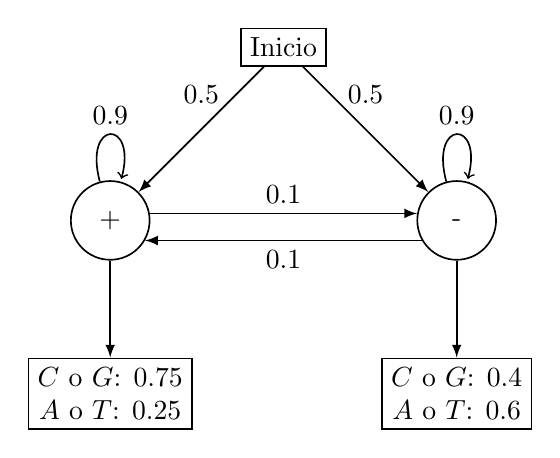
\begin{tikzpicture}[-latex ,auto , node distance =2.2 cm ,semithick, main/.style = {draw, circle, minimum size=1cm}] 
    \node[rectangle, draw, align=center] (1) {Inicio};
    \node[main] (2) [left of=1, below of=1] {+};
    \node[main] (3) [right of=1, below of=1] {-};
    \node[rectangle, draw, align=center] (4) [below of=2]{$C$ o $G$: 0.75\\$A$ o $T$: 0.25};
    \node[rectangle, draw, align=center] (5) [below of=3]{$C$ o $G$: 0.4\\$A$ o $T$: 0.6};

    \draw (1) -- node[above=0.2cm] {0.5} (2);
    \draw (1) -- node[above=0.2cm] {0.5} (3);
    \path (2) edge [loop above] node {0.9} (2);
    \draw (2.10) -- node[midway] {0.1} (3.170);
    \path (3) edge [loop above] node {0.9} (3);
    \draw (3. 210) -- node[midway] {0.1} (2.330);
    
    \draw (2) -- node[] {} (4);
    \draw (3) -- node[] {} (5);
\end{tikzpicture}
\caption{HMM sencillo para identificar islas CpG \cite{bioStudies}}
\end{figure}

Usando este modelo podemos utilizar el algoritmo de Viterbi para identificar islas CpG. Como ejemplo, consideramos la siguiente secuencia:

\seqsplit{TCTCGCTGCCGCCAACCCTCGGCGCCGTCGGGTTCGCCGCGGCTCTGATAAGTCCCGTTTATGGTACCCGGGCCGATCTCTGGTGGGAATCGGAGACCTGTGTACCCTGACGCATCCGTTTGTGTTCCCTACACGGCCGACGCAGACCGGGCGCGCGGCGCCACCCAACGAAGCCCGGGTATGGCACGTGCCCCAGGCGGTGCCCTACCCGTATTTCGGGACAAGTTCCCGGATCGGGTGAAAGTTAACGGAAGGATGCCAAGCAATAGCGGCCACAGGACCCGCCTGGCGACGCATGGACTGGATCCGGAGGTCTGGCCAACAGTTGATTTCATGGGTTACAGCCCCGGTGTAGATCCCCTCATGGTCTCCCGAACCGATTAGTTTGAAAACTGTATCTCCTGGCCGCCTAACAGGTATAAAGAGCCGGCTCACACTGGGGTGAGGGGGCGCGTGGCCCCCTT}


Para determinar si proviene de una isla CpG aplicamos el algoritmo de Viterbi utilizando funcionalidades de \textbf{hmmlearn}. Obtenemos el siguiente secuencia de estados:

\textbf{\seqsplit{+++++++++++++++++++++++++++++++++++++++++++-----------------------+++++++++++++++++++++++++++++++++++++++++++++++++++++++++++++++++++++++++++++++++++++++++++++++++++++++++++++++++++++++++++++++++++++++++++++++++---------------------------------------------------------++++++++++++++++++++++++++++++++++++++++++++++++++++-----------------------++++++++++++++++++++++++++++++++++++---------------------++++++++++---------------+++++++++++++++++++++++++++++++++++++++}}

Podemos usar este resultado para distinguir los estados correspondientes en la secuencia de observaciones:

\textcolor{blue}{\seqsplit{TCTCGCTGCCGCCAACCCTCGGCGCCGTCGGGTTCGCCGCGGC}}\textcolor{red}{\seqsplit{TCTGATAAGTCCCGTTTATGGTA}}\textcolor{blue}{\seqsplit{CCCGGGCCGATCTCTGGTGGGAATCGGAGACCTGTGTACCCTGACGCATCCGTTTGTGTTCCCTACACGGCCGACGCAGACCGGGCGCGCGGCGCCACCCAACGAAGCCCGGGTATGGCACGTGCCCCAGGCGGTGCCCTACCCG}}\textcolor{red}{\seqsplit{TATTTCGGGACAAGTTCCCGGATCGGGTGAAAGTTAACGGAAGGATGCCAAGCAATA}}\textcolor{blue}{\seqsplit{GCGGCCACAGGACCCGCCTGGCGACGCATGGACTGGATCCGGAGGTCTGGCC}}\textcolor{red}{\seqsplit{AACAGTTGATTTCATGGGTTACA}}\textcolor{blue}{\seqsplit{GCCCCGGTGTAGATCCCCTCATGGTCTCCCGAACCG}}\textcolor{red}{\seqsplit{ATTAGTTTGAAAACTGTATCT}}\textcolor{blue}{\seqsplit{CCTGGCCGCC}}\textcolor{red}{\seqsplit{TAACAGGTATAAAGA}}\textcolor{blue}{\seqsplit{GCCGGCTCACACTGGGGTGAGGGGGCGCGTGGCCCCCTT}}

Donde el color azul representa que las letras provienen de un estado + y el color rojo representa que provienen de un estado - como resultado de aplicar el algoritmo de Viterbi. Si analizamos las secuencias en rojo, podemos ver que contienen una proporción de $T$ o $A$ superior al de $50\%$. Pero en definitiva, tenemos una mayor proporción de estados + en la secuencia de estados resultante, lo que sugiere que la secuencia de observaciones puede provenir de una isla CpG.

\section{Alineamiento de pares de secuencias}
En análisis de secuencias, muchas veces es importante comparar dos secuencias para determinar si están funcionalmente relacionadas. Por ejemplo, genes con funciones similares en diferentes organismos suelen tener secuencias de ADN muy similares. Si un gen nuevo es suficientemente similar a otro gen de otro organismo cuya función es conocida, entonces es razonable esperar que el nuevo gen ejerza la misma función. Lo mismo ocurre con las proteínas, si se descubre una nueva proteína del que se desconoce su estructura tridimensional pero con una similitud sustancial entre su secuencia de aminoácidos y la secuencia de una proteína del que sí se conoce la estructura tridimensional, entonces es razonable esperar que la estructura de la nueva proteína sea de alguna forma similar al de la proteína conocida.

Para estudiar este problema, comenzamos estableciendo algunas notaciones. Vamos a considerar un par de secuencias, $x$ e $y$ de longitudes $n$ y $m$ respectivamente. Sea $x_i$ el $i$-ésimo símbolo de $x$ e $y_j$ el $j$-ésimo símbolo de $y$, estos símbolos pertenecen a un cierto alfabeto $\mathcal{A}$ que en el caso del ADN serán las $4$ bases $\{A,C,G,T\}$ y en el caso de las proteínas serán los $20$ aminoácidos.

Si sólo consideramos las secuencias originales el problema sería trivial: sólo existe un único alineamiento en el caso de que $n=m$ y en otro caso, el problema se reduciría en encontrar la mejor posición para incluir una secuencia en otra. El problema real se tiene en cuenta posibles inserciones de huecos (\textit{gaps}) en cualquiera de las dos secuencias, sin posibilidad de insertar hueco en ambas secuencias al mismo tiempo ni insertar dos huecos en diferentes secuencias de forma seguida, para obtener alineamientos entre símbolos iguales. Consideramos el siguiente ejemplo:

\begin{exampleth}
    Tomamos dos secuencias de ADN:
    \begin{center}
        $x=CACGAAT$, $y=AGTTCAA$
    \end{center}
    Podemos considerar un alineamiento entre estas dos secuencias como sigue:
    \[\begin{array}{c c c c c c c c c c}
        C & A & - & - & - & C & G & A & A & T \\
        - & A & G & T & T & C & - & A & A & -
    \end{array}\]
    donde cada $-$ representa un hueco.
\end{exampleth}

Como podemos apreciar en el ejemplo, las inserciones producen nuevos alineamientos a tener en cuenta. Para valorar estos alineamientos, se define una matriz de puntuaciones que asigna para cada alineamiento de símbolos un valor. Esta matriz se conoce usualmente como la matriz de sustitución, un ejemplo de matriz de sustitución para secuencias de ADN podría ser la siguiente:
\[
S=\begin{blockarray}{ccccc}
 & A & C & G & T \\
\begin{block}{c(cccc)}
  A & 10 & -3 & -2 & 1 \\
  C & -2 & 8 & 1 & -2 \\
  G & -3 & 1 & 9 & -3 \\
  T & 0 & -3 & -2 & 6\\
\end{block}
\end{blockarray}
 \]
En esta matriz, cada elemento representa la puntuación que obtendría un alineamiento entre el símbolo de la fila y el símbolo de la columna. Cada uno de estos valores, se puede calcular de la siguiente manera:
\[s(a,b)=\log\left(\dfrac{p_{ab}}{q_a\cdot q_b}\right)\]
siendo $a$ y $b$ elementos del alfabeto $\mathcal{A}$, $p_{ab}$ la probabilidad de que se produzca un emparejamiento entre $a$ y $b$ y $q_a$ la frecuencia relativa esperada de que se produzca un símbolo $a$ en una secuencia. 

Estos valores son relevantes pues afectan a la significación final del análisis: si tenemos un sistema de puntuación ajustado a la realidad, podremos afirmar con mayor seguridad las similitudes entre dos secuencias. Por esta razón, existen métodos para derivar estos valores a partir de datos conocidos y matrices de sustitución utilizadas ampliamente como las matrices PAM o BLOSUM.

Además de los alineamientos entre los símbolos del alfabeto, se tiene en cuenta también los alineamiento entre un símbolo y un hueco. Estos alineamientos tienen una puntuación negativa, lo que se conoce generalmente como penalizaciones por hueco (\textit{gap penalties}). El coste asociado a una consecución de huecos de longitud $g$ puede venir dado por una de las dos siguientes funciones lineares:
\[\gamma_1(g)=-gd \]
\[\gamma_2(g)=-d-(g-1)e\]
donde $d$ se considera la penalización por iniciar la secuencia de huecos y $e$ se considera la penalización por extender la secuencia, usualmente con un valor menor que $d$. Mientras que en $\gamma_1$ se trata todos los huecos por igual, en $\gamma_2$ se penaliza menos las secuencias de huecos con mayores longitudes. Esto es deseable cuando se prevé que las inserciones de varios huecos sean tan frecuentes como inserciones de un único hueco. En la práctica, los valores $d$ y $e$ se escogen empíricamente una vez elegido los valores de la matriz de sustitución.

Con estos elementos, podemos determinar el mejor alineamiento con huecos entre dos secuencias entendiéndolo como aquel con mayor puntuación dada la matriz de sustitución. Si consideramos las dos secuencias enteras, estaremos hablando del alineamiento global de pares de secuencias. Si lo que buscamos es el mejor alineamiento entre subsecuencias de $x$ e $y$, entonces estaremos hablando del alineamiento local.

Para nuestro estudio, vamos a centrarnos en el problema de alineamiento global. Este problema se puede resolver empleando el algoritmo de Needleman-Wunsch, un algoritmo de programación dinámica que garantiza encontrar el alineamiento óptimo entre dos secuencias con posibles huecos. Pero también podemos utilizar un tipo específico de HMM para resolver este problema, los \textit{Pair HMMs}.

\subsection{Pair HMM}
A diferencia de los HMMs que habíamos presentado hasta ahora, los \textit{pair HMMs} generan dos salidas en cada estado en lugar de uno. Por esta razón, podemos utilizar este modelo para el problema de alineamiento de pares. Existen distintas variaciones de este modelo, vamos a presentar el modelo ilustrado en \cite{Durbin}. 

%El espacio de salidas del modelo está compuesto por los posibles alineamientos que pueden haber: entre dos símbolos del alfabeto $\mathcal{A}$, entre un símbolo y un hueco o entre un hueco y un símbolo. En definitiva:
%\[\mathbb{V}=\{\mathcal{A}\times\mathcal{A}\}\cup \{\mathcal{A}\times -\} \cup \{-\times\mathcal{A}\} \]

El espacio de estados consiste principalmente en tres estados: en el estado $M$ se generan dos símbolos del alfabeto $\mathcal{A}$ mientras que en los estados $X$ e $Y$ se emite un símbolo de la salida correspondiente dejando un hueco en la otra. Llamaremos $p_{ab}$ a la probabilidad de que se emitan los símbolos $a$ y $b$ desde el estado $M$ y $q_{a}$ la probabilidad de emitir un símbolo $a$ y un hueco desde los estados $X$ e $Y$.

A los estado $X$ e $Y$ se les conocen como estados de inserción (o estado de inserción y eliminación en algunas literaturas, por ejemplo \cite{Marina}) y al estado $M$, el estado de alineamiento (\textit{match state}). 


Asumiendo que los procesos de salida son idénticos, existen dos parámetros para definir las probabilidades de transición entre estos estados: $\mu$ como probabilidad de pasar del estado $M$ a un estado de inserción ($X$ o $Y$) y $\epsilon$ como la probabilidad de permanecer en un estado de inserción.

Puesto que estamos tratando con secuencias espaciales en lugar de temporales, tiene sentido definir un estado de inicio y un estado de fin. Ambos estados son estados silenciosos, estados que no producen ninguna salida. El hecho de añadir un estado de inicio facilita posteriormente en la modificación de los algoritmos. Este estado sustituye la función de la distribución inicial, de modo que el modelo siempre empezará por el estado de inicio. Para este problema, podemos considerar que el estado de inicio tenga las mismas probabilidades de transición que $M$.

Por otro lado, al añadir un estado de fin necesitamos introducir un nuevo parámetro, la probabilidad de pasar a dicho estado desde los otros estados. Asumiendo que es la misma desde cualquier de los otros estados, llamamos a dicho parámetro $\tau$. Este valor influirá en la longitud media de los alineamientos generados por el modelo. Con estos elementos, tenemos el modelo que se muestra en la figura \ref{pairEjemplo}.

\begin{figure}
\centering
\begin{tikzpicture}[-latex ,auto , node distance =3.5 cm ,semithick, main/.style = {draw, circle, minimum size=1.2cm}] 
    \node[main] (1) {Inicio};
    \node[main] (2) [right of=1] {$M$};
    \node[main] (3) [right of=2, above=1.4 cm of 2] {$X$};
    \node[main] (4) [right of=2, below=1.4 cm of 2] {$Y$};
    \node[main] (5) [right of=3, below = 1.4cm of 3] {Fin};
    
    \path (1) edge [bend left, above, pos=0.7] node {$1-2\mu-\tau$} (2);
    \draw (1) edge [bend left=35] node {$\mu$} (3);
    \draw (1) edge [bend right=40] node {$\mu$} (4);
    \draw (1) edge [bend right=90] node {$\tau$} (5);
    
    \path (2) edge [distance=2cm, out=170, in=210, below, pos=0.7] node {$1-2\mu-\tau$} (2);
    \draw (2) edge [bend left=10] node {$\mu$} (3);
    \draw (2) edge [bend right=10, below] node {$\mu$} (4);
    \draw (2) -- node[midway, below] {$\tau$} (5);

    \path (3) edge [distance=2cm, out=330, in=30, right=1cm] node {$\epsilon$} (3);
    \draw (3) edge [bend left=10] node {$1-\epsilon-\tau$} (2);
    \draw (3) edge [bend right] node {$\tau$} (5);

    \path (4) edge [distance=2cm, out=10, in=70, right=1cm] node {$\epsilon$} (4);
    \draw (4) edge [bend right=10, right=0.1cm] node {$1-\epsilon-\tau$} (2);
    \draw (4) edge [bend right, below] node {$\tau$} (5);

    %\path (5) edge [distance=1cm, above] node {1} (5);
    
\end{tikzpicture}
\caption{Estructura de \textit{Pair HMM} \cite{Durbin}}
\label{pairEjemplo}
\end{figure}
Una vez conocido el modelo, podemos aplicar el algoritmo de Viterbi adaptado para encontrar el alineamiento óptimo. En este caso, la entrada consiste en dos secuencias $x=(x_1,\dots,x_n)$ e $y=(y_1,\dots,y_m)$ y la salida es la secuencia de estados que conduce al alineamiento óptimo. 

Utilizaremos los índices $i$ y $j$ para referirnos a los elementos de las secuencias $x$ e $y$. Puesto que $x_i$ e $y_j$ son elementos del alfabeto $\mathcal{A}$, usaremos la notación $p_{x_iy_j},\,q_{x_i},\,q_{y_j}$ para distinguir los alineamientos entre los símbolos y los posibles huecos de $x$ e $y$.

Recordemos que en el algoritmo original:
\[
    \delta_t(i)=\max_{(q_0,q_1\dots,q_{t-1})\in\mathbb{S}^t}P[\mathcal{X}_0^{t}=(q_0,q_1,\dots,q_{t-1},s_i),\mathcal{Y}_0^t=(O_0,\dots,O_t)]
\]

Y se calcula de la siguiente forma:
\begin{align*}
    &\delta_0(i)=b_{s_i}(O_0)\cdot\pi_i, \\
    &\delta_t(i)=\max_{j=1,\dots,N}\left(a_{ji}\cdot\delta_{t-1}(j)\right) \cdot b_{s_i}(O_t), &&1\leq i\leq N,\quad1\leq t\leq r. \tag{4.\arabic{Bio}}\label{viterbiOriginal}
\end{align*}

En este caso, sólo tenemos que calcular las variables relacionadas con los estados $M,\,X,\,$ e $Y$. El estado de inicio se representará también por el estado $M$ por simplicidad. Puesto que el estado fin es un estado silencioso y representa el final del alineamiento, tendrá un tratamiento especial. 

Usando los índices $i$ y $j$, la variable del algoritmo de Viterbi pasa a ser de forma $\delta_{i,j}(s)$ con $s\in\{M,X,Y\}$. Esta variable tiene el mismo significado que en el caso general: es la probabilidad de la secuencia de estado más probable terminado en el estado $s$, habiendo considerado hasta las posiciones $i$ y $j$ de las secuencias de entrada. Por lo tanto, el cálculo es idéntico al caso general, sustituyendo el índice temporal por los índices $i$ y $j$.

Concretamente, inicializamos el algoritmo asignando los siguientes valores:
\[\delta_{0,0}(M)=1\]
\[\delta_{0,j}(X)=\delta_{i,0}(Y)=0,\qquad  0\leq i\leq n, \, 0\leq j \leq m\]
\[\delta_{0,j}(M)=\delta_{i,0}(M)=0,\qquad  1\leq i\leq n, \, 1\leq j \leq m\]


El primer caso se debe a que siempre empezamos en el estados de inicio (que hemos representado en este caso por el estado $M$) y al ser silencioso podemos asumir que tiene la probabilidad de emisión $1$. Los otros casos se deben a que son situaciones imposibles. Por ejemplo, $\delta_{0,1}(X)$ es la probabilidad de que se haya considerado $y_1$ y ningún símbolo de $x$ habiendo tomado como último estado el estado $X$. Esto contradice con la propia definición de $X$, pues en dicho estado siempre se emite un símbolo de $x$ con un hueco en $y$.

El resto de las variables se calculan de forma similar que en \eqref{viterbiOriginal}, iremos por casos:
\begin{itemize}
    \item $\delta_{i,j}(M)$ indica que se ha alineado $x_i$ e $y_j$ tomando como último estado el estado $M$. Además, aplicando recursividad, tenemos que encontrar la probabilidad de la secuencia más probable habiendo considerado hasta las posiciones $i-1$ y $j-1$ terminado en un estado $s$ y considerar la transición de $s$ a $M$:
    \[\delta_{i,j}(M)=p_{x_iy_j}\cdot \max
    \begin{cases}
        (1-2\mu-\tau)\cdot\delta_{i-1,j-1}(M) \\
        (1-\epsilon-\tau)\cdot\delta_{i-1,j-1}(X) \\
        (1-\epsilon-\tau)\cdot\delta_{i-1,j-1}(Y)
    \end{cases} \quad 1\leq i\leq n, \, 1\leq j \leq m\] 

    \item $\delta_{i,j}(X)$ indica que se ha emitido $x_i$ y un hueco tomando como último estado el estado $X$. Puesto que en este caso no se emite ningún símbolo de $y$, quiere decir que $y_j$ ya había sido emitido anteriormente. Como no es posible pasar del estado $Y$ al $X$, existen dos posibilidades: el alineamiento entre $x_{i-1}$ e $y_j$ o el alineamiento entre $x_k$ e $y_j$ con $k<i-1$. Este último caso implicaría la emisión de $x_{i-1}$ con un hueco, por lo tanto:
    \[\delta_{i,j}(X)=q_{x_i}\cdot \max 
    \begin{cases}
        \mu\cdot\delta_{i-1,j}(M) \\
        \epsilon\cdot\delta_{i-1,j}(X) 
    \end{cases} \qquad 1\leq i\leq n, \, 0\leq j \leq m\]

    \item $\delta_{i,j}(Y)$ se calcula de mismo modo que $\delta_{i,j}(X)$:
    \[\delta_{i,j}(Y)=q_{y_j}\cdot \max 
    \begin{cases}
        \mu\cdot\delta_{i,j-1}(M) \\
        \epsilon\cdot\delta_{i,j-1}(Y) 
    \end{cases} \qquad 0\leq i\leq n, \, 1\leq j \leq m \]
\end{itemize}
Finalmente, se calcula:
\[\delta(Fin)=\tau\cdot\max\{\delta_{n,m}(M),\,\delta_{n,m}(X),\,\delta_{n,m}(Y)\}\]
Para obtener la secuencia óptima mantenemos el estado correspondiente al argumento máximo de cada variable y lo recuperamos desde $\delta(Fin)$ del mismo modo que en el algoritmo original. Para evitar el problema de convergencia a $0$, basta aplicar logaritmo a las variables tal como habíamos en la versión original.

\begin{exampleth}
    Introducir ejemplo programado aquí
\end{exampleth}

Una de las ventajas que nos proporciona la utilización de \textit{pair HMM} respecto a la programación dinámica, es que ahora podemos calcular la probabilidad de que dos secuencias estén relacionadas según el modelo independientemente del alineamiento. Lo hacemos considerando todos los posibles alineamientos:
\[P[x,y]=\sum_{Alineamiento\, Q}P[x,y,Q]\]
Para calcular esta suma adaptamos el algoritmo de avance a este modelo. La variable de avance se puede calcular de forma recursiva similar a la variable de Viterbi, pero sumando las variables previos en lugar de calcular el máximo.

\begin{exampleth}
    Introducir ejemplo programado aquí
\end{exampleth}

\section{Familias de secuencias}
En el apartado anterior hemos visto cómo podemos alinear dos secuencias de ADN o de proteínas para determinar si están relacionados. En general, secuencias biológicas con funciones similares forman familias. Para caracterizar las propiedades de una familia, se acude al alineamiento múltiple de secuencias de la familia. Una vez obtenido dicho alineamiento, podemos determinar si una nueva secuencia $x$ pertenece a la familia correspondiente. Y en caso afirmativo, concluir que tiene una determinada funcionalidad. 

Para modelar las similitudes resultantes del alineamiento, podemos modelarlo mediante un tipo particular de HMM, llamado \textit{profile HMM}. En este apartado, vamos a asumir que tenemos dado el alineamiento múltiple de secuencias de una familia y vamos a presentar la forma de construir el \textit{profile HMM} correspondiente. 

A diferencia de los HMMs generales, los \textit{profile HMMs} tiene una estructura estrictamente linear y no cíclica. El primer paso para construir el modelo es determinar su longitud. Para ello, necesitamos separar el alineamiento en dos posibles regiones: la región de alineamiento, que está formada por posiciones cuyos elementos son mayoritariamente símbolos y la región de inserción formada por posiciones con una alta frecuencia de huecos. Aunque existen diferentes criterios, lo usual es que posiciones cuyos huecos son más de la mitad de los elementos formen parte de la región de inserción y en caso contrario, formen parte de la región de alineamiento. Veamos con el siguiente ejemplo:

\begin{exampleth} \label{alineamientoMúltiple}
    \[\begin{array}{c c c c c c}
        T & A & - & -  & T & C \\
        T & A & G & -  & T & C \\
        T & A & G & A  & - & C \\
        - & A & G & -  & T & G \\
        \textcolor{blue}{M} & \textcolor{blue}{M} & \textcolor{blue}{M} & \textcolor{red}{I} & \textcolor{blue}{M} & \textcolor{blue}{M}
    \end{array}\]    
    Las posiciones con \textcolor{blue}{$M$} en última fila indica que pertenecen a la región de alineamiento mientras que la posición con \textcolor{red}{$I$} indica que pertenece a la región de inserción.
\end{exampleth}

Una vez identificada las regiones, la longitud del modelo viene dada por el número de posiciones que forman parte de la región de alineamiento. Conocida la longitud, el siguiente paso es construir el espacio de estados, que está principalmente constituido por $3$ tipos de estados: los estados de alineamiento $M_k$, los estados de inserción $I_k$ y los estados de eliminación $D_k$. Cada uno de de los índices $k$, corresponde con la $k$-ésima posición dentro de la región de alineamiento comenzando desde $1$. 
Para el ejemplo \ref{alineamientoMúltiple} tenemos:
\[\begin{array}{c c c c c c c}
   & T & A & - & -  & T & C \\
   & T & A & G & -  & T & C \\
   & T & A & G & A  & - & C \\
   & - & A & G & -  & T & G \\
   \hline
  k= & 1 & 2 & 3 & & 4 & 5 
\end{array}\]   
A partir de la longitud $n$, construimos un HMM trivial formado por los estados de alineamiento $M_k$ con $k=1,\dots, n$ y probabilidades de transición $1$ al siguiente estado $M_{k+1}$. Los estados $M_k$ representan el caso de que un símbolo de $x$ se alinee con el símbolo más frecuente de la posición correspondiente. Las probabilidades de emisión de $M_k$ corresponden con las frecuencias relativas de cada símbolo en la posición $k$-ésima del alineamiento. También consideramos los estados de inicio y fin, con los mismos significados que en el caso de \textit{pair HMM} pero con probabilidades de transición triviales. Para el ejemplo \ref{alineamientoMúltiple} tenemos el siguiente HMM:

\begin{figure}[H]
\centering
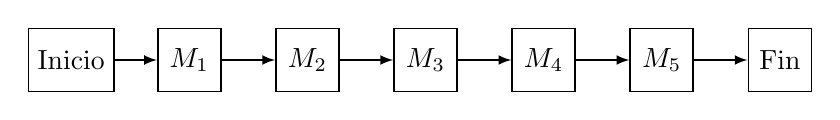
\begin{tikzpicture}[-latex ,auto, node distance =1.5 cm ,semithick, main/.style = {draw, rectangle, minimum size=0.8cm}] 
    \node[main] (1) {Inicio};
    \node[main] (2) [right of=1] {$M_1$};
    \node[main] (3) [right of=2] {$M_2$};
    \node[main] (4) [right of=3] {$M_3$};
    \node[main] (5) [right of=4] {$M_4$};
    \node[main] (6) [right of=5] {$M_5$};
    \node[main] (7) [right of=6] {Fin};
    
    \draw (1) -- node[] {} (2);
    \draw (2) -- node[] {} (3);
    \draw (3) -- node[] {} (4);
    \draw (4) -- node[] {} (5);
    \draw (5) -- node[] {} (6);
    \draw (6) -- node[] {} (7);

    
\end{tikzpicture}
\caption{HMM trivial a partir del ejemplo \ref{alineamientoMúltiple}}
\end{figure}

A partir del modelo trivial, añadimos los estados $I_k$ y $D_k$. Los estados $I_k$ modelan las inserciones, emisiones de símbolos adicionales a los $n$ símbolos emitidos por el modelo trivial. En otras palabras, cada inserción representa el alineamiento de un símbolo en una posición fuera de la región de alineamiento y formada mayoritariamente o totalmente por huecos. En este caso, $k$ indica la última posición de la región de alineamiento anterior a la inserción. Para modelar posibles inserciones anteriores a cualquier alineamiento de símbolos, añadimos un estado $I_0$. Cada estado de inserción está asociado a $3$ transiciones posibles: $M_k\rightarrow I_k$ que representa la inserción tras un alineamiento, $I_k\rightarrow I_k$ para permitir inserciones múltiples y la transición $I_k\rightarrow M_{k+1}$ para un nuevo alineamiento. 

Por otra parte, los estados $D_k$ modelan las eliminaciones, emisiones de huecos en la posición $k$ de la región de alineamiento. Cada estado tiene $4$ transiciones posibles: $M_{k-1}\rightarrow D_k$ representando la eliminación en la posición $k$ de la región de alineamiento, $D_k \rightarrow D_{k+1}$ para permitir eliminaciones múltiples, $D_k\rightarrow M_{k+1}$ para alinear después de una eliminación. 

Además, permitimos las transiciones $D_k \rightarrow I_k$ para inserciones tras eliminar e $I_{k}\rightarrow D_{k+1}$ para eliminaciones tras insertar. Éstas transiciones son muy poco probables, pero los añadimos pues dejándolos fuera puede generar problemas a la hora de construir el modelo.

Tomando el alineamiento del ejemplo \ref{alineamientoMúltiple}, añadiendo los estados y transiciones al modelo trivial, obtenemos el siguiente \textit{profile HMM}:

\begin{figure}[H]
\centering
    \begin{tikzpicture}[-latex ,auto, node distance =2 cm, semithick, main/.style = {draw, rectangle, minimum size=0.8cm},
        rombo/.style = {draw, diamond, minimum size=0.8cm}, circulo/.style = {draw, circle, minimum size=0.8cm}] 
        \node[main] (1) {Inicio};
        \node[main] (2) [right of=1] {$M_1$};
        \node[main] (3) [right of=2] {$M_2$};
        \node[main] (4) [right of=3] {$M_3$};
        \node[main] (5) [right of=4] {$M_4$};
        \node[main] (6) [right of=5] {$M_5$};
        \node[main] (7) [right of=6] {Fin};
    
        \node[rombo] (8)  [above of=1] {$I_0$};
        \node[rombo] (9) [right of=8] {$I_1$};
        \node[rombo] (10) [right of=9] {$I_2$};
        \node[rombo] (11) [right of=10] {$I_3$};
        \node[rombo] (12) [right of=11] {$I_4$};
        \node[rombo] (13) [right of=12] {$I_5$};

        \node[circulo] (14) [above of=9] {$D_1$};
        \node[circulo] (15) [right of=14] {$D_2$};
        \node[circulo] (16) [right of=15] {$D_3$};
        \node[circulo] (17) [right of=16] {$D_4$};
        \node[circulo] (18) [right of=17] {$D_5$};
        
        \draw (1) -- node {} (2);
        \draw (1) -- node {} (8);
        \draw (1) -- node {} (14);

        
        \draw (2) -- node {} (3);
        \draw (2) -- node {} (9);
        \draw (2) -- node {} (15);


        \draw (3) -- node {} (4);
        \draw (3) -- node {} (10);
        \draw (3) -- node {} (16);

        
        \draw (4) -- node {} (5);
        \draw (4) -- node {} (11);
        \draw (4) -- node {} (17);
        
        \draw (5) -- node {} (6);
        \draw (5) -- node {} (12);
        \draw (5) -- node {} (18);
        
        \draw (6) -- node {} (7);
        \draw (6) -- node {} (13);

        \path (8) edge [distance=0.5cm, out=155, in=205] node {} (8);
        \draw (8) -- node {} (2);
        \draw (8) -- node {} (14);

        
        \path (9) edge [distance=0.5cm, out=155, in=205] node {} (9);
        \draw (9) -- node {} (3);
        \draw (9) -- node {} (15);

        
        \path (10) edge [distance=0.5cm, out=155, in=205] node {} (10);
        \draw (10) -- node {} (4);
        \draw (10) -- node {} (16);

        \path (11) edge [distance=0.5cm, out=155, in=205] node {} (11);
        \draw (11) -- node {} (5);
        \draw (11) -- node {} (17);

        \path (12) edge [distance=0.5cm, out=155, in=205] node {} (12);
        \draw (12) -- node {} (6);
        \draw (12) -- node {} (18);

        \path (13) edge [distance=0.5cm, out=155, in=205] node {} (13);
        \draw (13) -- node {} (7);

        \draw (14) -- node {} (15);
        \draw (14) -- node {} (9);
        \draw (14) -- node {} (3);
        
        \draw (15) -- node {} (16);
        \draw (15) -- node {} (10);
        \draw (15) -- node {} (4);

        \draw (16) -- node {} (17);
        \draw (16) -- node {} (11);
        \draw (16) -- node {} (5);
        
        \draw (17) -- node {} (18);
        \draw (17) -- node {} (12);
        \draw (17) -- node {} (6);
        
        \draw (18) -- node {} (7);
        \draw (18) -- node {} (13);
    \end{tikzpicture}
\caption{\textit{Profile HMM} a partir del ejemplo \ref{alineamientoMúltiple}}
\label{profileHMMFinal}
\end{figure}

Determinada la estructura del modelo, ahora necesitamos hallar las probabilidades de transición y de emisión. Con los estados que hemos definido, conocemos para cada una de las secuencias del alineamiento múltiple, la secuencia de estados que la produce. Por lo tanto, podemos estimar las probabilidades contando las transiciones y las emisiones de símbolos de todas las secuencias de estados y calcular las frecuencias relativas correspondientes. Para permitir probabilidades de transiciones o emisiones que no han sido observadas en el alineamiento original, añadimos un valor ponderado denominado pseudoconteo a los recuentos para evitar probabilidades iguales a cero. Este valor depende de la probabilidad que estamos calculando y del conocimiento que tenemos sobre el problema, el más simple posible es añadir $1$ a todas las observaciones. Veamos a continuación un ejemplo utilizando esta aproximación:

\begin{exampleth}
    Volvemos a tomar el alineamiento múltiple del ejemplo \ref{alineamientoMúltiple} con el modelo correspondiente a la figura \ref{profileHMMFinal}. En primer lugar vamos a determinar los estados que generan cada secuencia. Para evitar confusiones, pondremos $M_0$ para representar al inicio y $M_6$ para representar al fin. 
    \[\begin{array}{c c c c c c c c c}
       & T & A & - & -  & T & C & \implies &  M_0\, M_1\, M_2\,  D_3\,  M_4\,  M_5\,  M_6 \\
       & T & A & G & -  & T & C & \implies &  M_0\,  M_1\,  M_2\,  M_3\,  M_4\,  M_5\,  M_6 \\
       & T & A & G & A  & - & C & \implies &  M_0\,  M_1\,  M_2\,  M_3\,  I_3\,  D_4\,  M_5\,  M_6 \\
       & - & A & G & -  & T & G & \implies &  M_0 \,  D_1 \,  M_2 \,  M_3\,  M_4 \,  M_5 \,  M_6  \\
       \hline
       k= & 1 & 2 & 3 & & 4 & 5 & &
   \end{array}\]   
    Contamos ahora las frecuencias de cada símbolo en los estados $M_k$ e $I_k$, no es necesario calcular para los $D_k$ pues siempre emiten un hueco.

\begin{table}[H]
    \begin{minipage}{.5\linewidth}
        \centering
        \begin{tabular}{|c | C | C | C | C|}
             \hline
             & A & C & G & T \\
             \hline
             $M_1$ & 0 & 0 & 0 & 3 \\
             \hline
             $M_2$ & 4 & 0 & 0 & 0 \\
             \hline
             $M_3$ & 0 & 0 & 3 & 0 \\ 
             \hline
             $M_4$ & 0 & 0 & 0 & 3 \\
             \hline
             $M_5$ & 0 & 3 & 1 & 0 \\
             \hline
        \end{tabular}
        \caption{Emisiones desde $M_k$}
    \end{minipage}%
    \begin{minipage}{.5\linewidth}
        \centering
        \begin{tabular}{|c | C | C | C | C|}
            \hline
            & A & C & G & T \\
            \hline
            $I_0$ & 0 & 0 & 0 & 0 \\
            \hline
            $I_1$ & 0 & 0 & 0 & 0 \\
            \hline
            $I_2$ & 0 & 0 & 0 & 0 \\
            \hline
            $I_3$ & 1 & 0 & 0 & 0 \\ 
            \hline
            $I_4$ & 0 & 0 & 0 & 0 \\
            \hline
            $I_5$ & 0 & 0 & 0 & 0 \\
            \hline
        \end{tabular}
        \caption{Emisiones desde $I_k$}
    \end{minipage}
\end{table}
Para las transiciones entre estados, tenemos las siguientes frecuencias donde cada $k$ representa el índice del estado que inicia la transición:
\begin{table}[H]
    \centering
    \begin{tabular}{|c|C|C|C|C|C|C|C|}
        \hline
        $k$ & 0 & 1 & 2 & 3 & 4 & 5  \\
        \hline
        $M\rightarrow M$ & 3 & 3 & 3 & 2 & 3 & 4\\
        $M\rightarrow D$ & 1 & 0 & 1 & 0 & 0 & - \\
        $M\rightarrow I$ & 0 & 0 & 0 & 1 & 0 & 0 \\
        \hline
        $I\rightarrow M$ & 0 & 0 & 0 & 0 & 0 & 0 \\
        $I\rightarrow D$ & 0 & 0 & 0 & 1 & 0 & - \\
        $I\rightarrow I$ & 0 & 0 & 0 & 0 & 0 & 0 \\
        \hline
        $D\rightarrow M$ & - & 1 & 0 & 1 & 1 & 0 \\
        $D\rightarrow D$ & - & 0 & 0 & 0 & 0 & - \\
        $D\rightarrow I$ & - & 0 & 0 & 0 & 0 & 0 \\
        \hline
    \end{tabular}
    \caption{Frecuencias de transiciones}
\end{table}
Como podemos ver, hay muchas transiciones y emisiones con frecuencia cero, para evitar probabilidades iguales a cero, sumamos $1$ a todas las frecuencias y calculamos las probabilidades:
\begin{table}[H]
    \begin{minipage}{.5\linewidth}
        \centering
        \begin{tabular}{|c | C | C | C | C|}
            \hline
            & A & C & G & T \\
            \hline
            $M_1$ & 1/7 & 1/7 & 1/7 & 4/7 \\
            \hline
            $M_2$ & 5/8 & 1/8 & 1/8 & 1/8 \\
            \hline
            $M_3$ & 1/7 & 1/7 & 4/7 & 1/7 \\ 
            \hline
            $M_4$ & 1/7 & 1/7 & 1/7 & 4/7 \\
            \hline
            $M_5$ & 1/8 & 1/2 & 1/4 & 1/8 \\
            \hline
        \end{tabular}
        \caption{Probabilidades de emisión de $M_k$}
    \end{minipage}%
    \begin{minipage}{.5\linewidth}
        \centering
        \begin{tabular}{|c | C | C | C | C|}
            \hline
            & A & C & G & T \\
            \hline
            $I_0$ & 1/4 & 1/4 & 1/4 & 1/4 \\
            \hline
            $I_1$ & 1/4 & 1/4 & 1/4 & 1/4 \\
            \hline
            $I_2$ & 1/4 & 1/4 & 1/4 & 1/4 \\
            \hline
            $I_3$ & 2/5 & 1/5 & 1/5 & 1/5 \\ 
            \hline
            $I_4$ & 1/4 & 1/4 & 1/4 & 1/4 \\
            \hline
            $I_5$ & 1/4 & 1/4 & 1/4 & 1/4 \\
            \hline
        \end{tabular}
        \caption{Probabilidades de emisión de $I_k$}
    \end{minipage}
\end{table}

\begin{table}[H]
    \centering
    \begin{tabular}{|c|C|C|C|C|C|C|C|}
        \hline
        $k$ & 0 & 1 & 2 & 3 & 4 & 5  \\
        \hline
        $M\rightarrow M$ & 4/7 & 2/3 & 4/7 & 1/2 & 2/3 & 5/6\\
        $M\rightarrow D$ & 2/7 & 1/6 & 2/7 & 1/6 & 1/6 & - \\
        $M\rightarrow I$ & 1/7 & 1/6 & 1/7 & 1/3 & 1/6 & 1/6 \\
        \hline
        $I\rightarrow M$ & 1/3 & 1/3 & 1/3 & 1/4 & 1/3 & 1/2 \\
        $I\rightarrow D$ & 1/3 & 1/3 & 1/3 & 1/2 & 1/3 & - \\
        $I\rightarrow I$ & 1/3 & 1/3 & 1/3 & 1/4 & 1/3 & 1/2 \\
        \hline
        $D\rightarrow M$ & - & 1/2 & 1/3 & 1/2 & 1/2 & 1/2 \\
        $D\rightarrow D$ & - & 1/4 & 1/3 & 1/4 & 1/4 & - \\
        $D\rightarrow I$ & - & 1/4 & 1/3 & 1/4 & 1/4 & 1/2 \\
        \hline
    \end{tabular}
    \caption{Probabilidades de transición}
\end{table}
    
\end{exampleth}